\documentclass[11pt,a4paper]{report}
\usepackage[utf8]{inputenc}
\usepackage{amsmath}
\usepackage{graphicx}
\usepackage{gensymb}
\usepackage{array}
\usepackage{multirow}

\usepackage{minted}
\makeatletter
\expandafter\def\csname PYGdefault@tok@err\endcsname{\def\PYGdefault@bc##1{{\strut ##1}}}
\makeatother

\usepackage{tikz}
\usetikzlibrary{arrows,positioning,calc}
\usepackage{tkz-graph}
\tikzset{
    %Define standard arrow tip
    >=stealth',
    % Define arrow style
    pil/.style={
           ->,
           thick,
           shorten <=2pt,
           shorten >=2pt,}
}
\usepackage{geometry}
\geometry{
    left=2cm,
    right=0.64cm,
    top=0.64cm,
    bottom=2cm
}
\usetikzlibrary{positioning}
\usepackage{geometry}
\geometry{
    left=2cm,
    right=0.64cm,
    top=0.64cm,
    bottom=2cm
}
\usepackage{multicol}
\setlength{\columnsep}{1cm}
\graphicspath{ {images/} }

\newcommand*{\titleGM}{\begingroup % Create the command for including the title page in the document
\hbox{ % Horizontal box
\hspace*{0.2\textwidth} % Whitespace to the left of the title page
\rule{1pt}{\textheight} % Vertical line
\hspace*{0.05\textwidth} % Whitespace between the vertical line and title page text
\parbox[b]{0.75\textwidth}{ % Paragraph box which restricts text to less than the width of the page

{\noindent\Huge\bfseries Distributed System \\[0.5\baselineskip] Summary} \\ % Title
[2\baselineskip]
{\large \textit{Don't expect everything here}}\\[4\baselineskip] % Tagline or further description
{\Large \textsc{Andy Chong Chin Shin}} % Author name

\vspace{0.5\textheight} % Whitespace between the title block and the publisher

}}
\endgroup}

\begin{document}

\pagenumbering{gobble}
\titleGM

\begin{multicols*}{2}
\tableofcontents
\end{multicols*}

\pagenumbering{arabic}
\setcounter{page}{1}
\chapter{Characterisation of Distributed Systems and System Models}

\begin{multicols*}{2}

\noindent Distributed System (DS) is a set of networked computers that communicate and coordinate their actions only by passing messages.

\noindent Internet is a very large distributed system that enables users to make use of services from everywhere

\section{Fundamental Characteristics of DS}

\noindent Concurrency: add more computers to increase capacity, and hence higher performance \\

\noindent Loosely coupled: no global clock and no global shared memory \\

\noindent Independent failures: any computer and subnetwork can fail at anytime, can be more fault-tolerant than stand-alone systems

\section {Main Motivation of DS: Resource Sharing}

\noindent Resources are shared by using services. Service is a distinct part of a computer system providing accesses to the managed resources \\

\noindent For resource sharing works, we must define:
\begin{itemize}
    \item Content and format of resources
    \item Naming and address
    \item Communication infrastructures
\end{itemize}

\section{Issues and Problems in DS}

\noindent Heterogeneity: hardware and software components are not identical, such as networks, endian formats, operating systems and programming languages\\

\noindent Scalability: remain effective when resources and users increase. This can be achieve by caching and replication of data and deploying multiple servers. We prefer decentralised design to avoid performance bottlenecks. \\

\noindent Failure handling: can be achieved by detecting, masking, tolerating, and recovery of failure

\section{Architecture Models}

\noindent Architectural model defines components, functions, placement of components, and relationship between components.

\subsection{Software and Hardware Layers}

\begin{center}
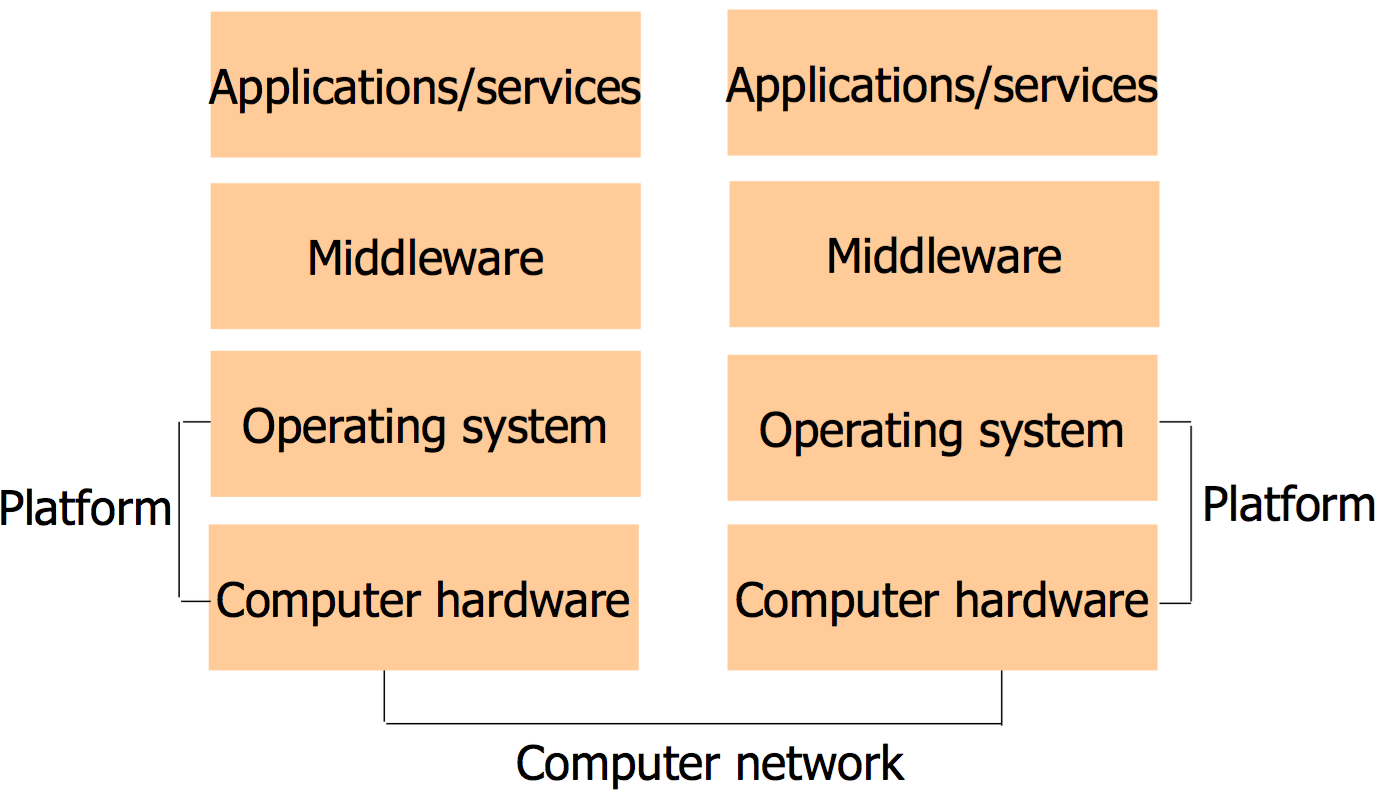
\includegraphics[width=8cm]{sw-hw-layers}
\end{center}

\noindent Platform provides system’s programming interface that facilitates communication and coordination between processes\\ 

\noindent Middleware masks heterogeneity and provide a convenient programming model. It provides generic services to application.

\subsection{Client-server Model}

\noindent $M$ servers work together for $N$ clients, so there is a division of work among $M$ servers. These servers need partitioning of data or function and replication of data or function.

\subsection{Peer-to-peer Model}

\noindent All processes play similar roles as clients and servers. The interact cooperatively as peers to perform distributed computation 

\section{Fundamental Models}

\noindent Fundamental model is formal description of common and intrinsic properties in architectural model. It makes exact claims by logical analysis and mathematical proof. 

\subsection{Interaction Model}

\noindent Synchronous distributed system assumes upper and lower bounds on processing time, transmission time, and clock drift rate. We can infer properties, such as using timeouts to detect failures.\\

\noindent Asynchronous distributed system assumes no bounds on processing time, transmission time and clock drift rate.

\subsection{Failure Model}

\noindent Failure model defines the ways in which failures may occur \\

\noindent Omission failure: a process or communication channel fails to perform actions it is supposed to do. \\

\noindent Arbitrary / Byzantine Failure: arbitrarily omit intended processing steps and take unintended processing steps.

\end{multicols*}

\chapter{Interprocess Communication}

\begin{multicols*}{2}
\section{External Data Representation}

\noindent External Data representation is an agreed standard for representation of data structures and primitive values. Data structure must be flattened before transmission and rebuilt on arrival. \\

\noindent Marshalling converts data items into the form suitable for transmission. Unmarshalling disassembles a message on arrival and restore data items

\subsection{CORBA’s Common Data Representation (CDR)}

\noindent Big / little-endian handling: transmit in sender’s ordering and the recipient translates\\

\noindent Example, flatten a \verb|Person| struct, with \verb|name| (string), \verb|place| (string) and \verb|year| (long) attributes, with value \verb|{“Smith”, “London”, 1934}|:\\

\begin{center}
\begin{tabular}{ |m{2cm}|c|p{4cm}| } 
    \hline
    Index in sequence of bytes & 4 bytes & Description \\
    \hline 
    0-3   & 5           & length of string \\
    4-7   & \verb|Smit| & \\
    8-11  & \verb|h___| & padded to flush on word boundary \\
    12-15 & 6           & length of string \\
    16-19 & \verb|Lond| & \\
    20-23 & \verb|on__| & padded to flush on word boundary \\
    24-27 & 1934        & \\
    \hline
\end{tabular}
\end{center}

\noindent Assumption: sender and recipient have common knowledge of the order and types of the data items

\subsection{Java Object Serialisation}

\noindent Assumption: the process doing deserialisation has no prior knowledge of the object types in the serialised form\\

\noindent Format: class information, types and names of instance variables, value of instance variables. \\

\noindent Each class is given a handle and no class is written more than once\\

\noindent Example, flatten a \verb|Person| struct, with \verb|name| (string), \verb|place| (string) and \verb|year| (long) attributes, with value \verb|{“Smith”, “London”, 1934}|:\\

\begin{center}
\begin{tabular}{ |p{1.8cm}|p{1.8cm}|p{1.8cm}|p{1.8cm}| } 
    \hline
    Person & \multicolumn{2}{p{3.6cm}|}{8 bytes version number} & h0 (class handle) \\
    \hline
    3 (number of fields) & int year & string name & string place \\
    \hline
    1934 & 5 Smith & 6 London & h1 (object handle) \\
    \hline
\end{tabular}
\end{center}

\section{Client-Server Communication}

\noindent Validity: the message reaches the destination\\

\noindent Integrity: the message received is identical to the one sent, and no message is delivered more than once

\subsection{Request-Reply Protocol over UDP}

\noindent Message is transmitted without acknowledgements or retires. \\

\noindent UDP is not a reliable communication service:

\begin{itemize}
    \item Integrity: use checksum to detect corrupt packets
    \item Validity: Message validity is not guarantee because it suffers communication omission failures.
\end{itemize}

\noindent To build reliable request-reply protocols over UDP, client uses timeouts when waiting for server’s reply and sends request repeatedly after timeout

\begin{center}
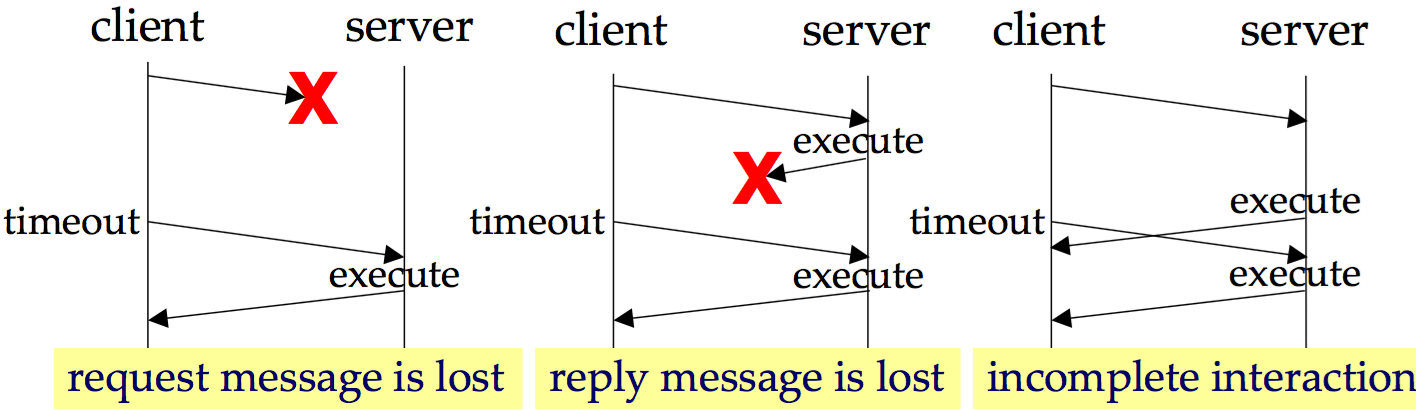
\includegraphics[width=8cm]{udp-interac}
\end{center}

\subsection{Request-Reply Protocol over TCP}

\noindent Message is transmitted with acknowledgement and retries. It is connection-oriented: a connection must be setup before any data are transferred.\\

\noindent TCP is a reliable communication service:

\begin{itemize}
    \item Integrity: use checksums to detect corrupt packets; use sequence numbers to detect duplicate packets
    \item Validity: received packets are acknowledged; use timeouts and retransmission to deal with lost packets.
\end{itemize}

\noindent Reducing Overhead: reuse a single TCP connection to send multiple requests

\subsection{Idempotent and Non-idempotent Operation}

\noindent Idempotent operations: can be performed repeatedly with the same effect as if performed exactly once\\

\noindent Non-idempotent operations: if performed repeatedly have different effects from if performed exactly once


\end{multicols*}

\chapter{Distributed Objects and Remove Invocation}
\begin{multicols*}{2}

\noindent Remote objects are objects that can receive remote invocations\\

\noindent Remote method invocation means method invocation between objects in different processes\\

\noindent Remote object reference is use to uniquely identify an object throughout a distributed system\\

\noindent Remote Interface: each remote object has a remote interface specifying the methods that can be invoked remotely

\section{Invocation Semantics}

\scriptsize
\begin{center}
\begin{tabular}{ |m{2cm}|p{1.7cm}|p{1.7cm}|p{1.7cm}| } 
    \hline
    \multirow{2}{2cm}{\begin{center}Invocation Semantics\end{center}} & \multicolumn{3}{p{5.1cm}|}{Fault Tolerance Measures} \\ \cline{2-4}
    & Retransmit request message & Duplicate filtering & Re-execute method or retransmit reply \\
    \hline
    Maybe\newline  & No  & N/A & N/A \\
    \hline
    At-least-once  & Yes & No  & Re-execute method \\
    \hline
    At-most-once   & Yes & Yes & Retransmit reply \\
    \hline
\end{tabular}
\end{center}
\normalsize

\section{Architecture of RMI}

\begin{center}
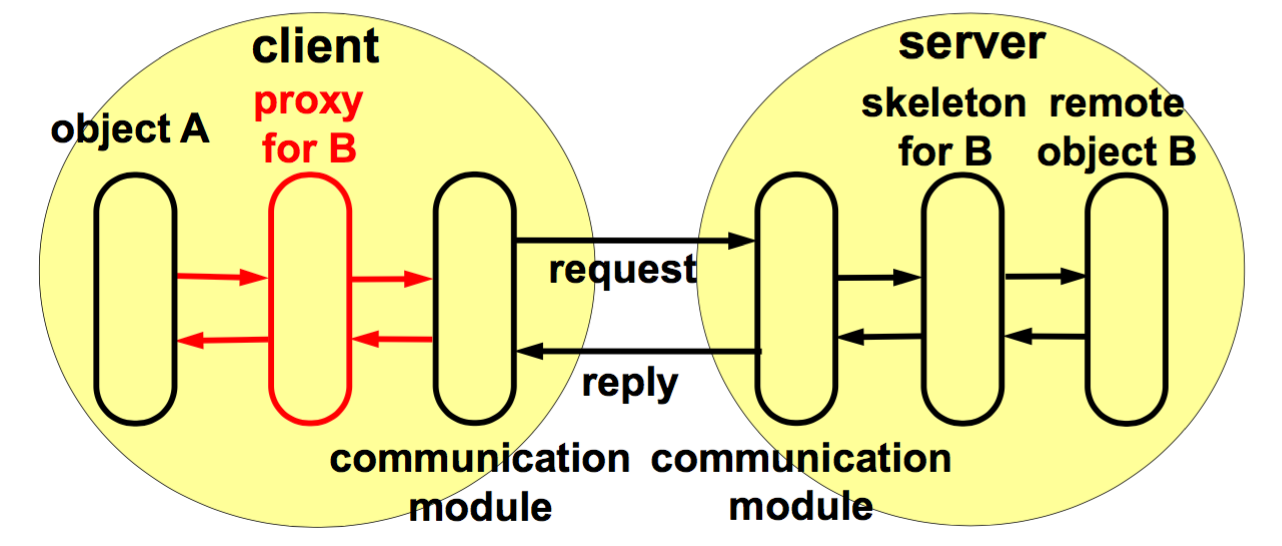
\includegraphics[width=8cm]{rmi-architecture}
\end{center}

\noindent One proxy for each class of remote objects. It marshals arguments and unmarshals results\\

\noindent Communication modules transmit request and reply message between client and server\\

\noindent One skeleton for each class of remote objects. It unmarshals arguments, invokes the corresponding method in the remote object, and marshals results\\

\noindent Binder is a name service that maintains mappings from object names to remote object references.

\section{Java RMI Architecture}

\noindent Step 1: Design the remote interface\\

\noindent Step 2: Design the servant class to implement the methods specified in the remote interface\\

\noindent Step 3: Design the server class to create remote objects and register then in RMI registry\\

\noindent Step 4: Design the client  class to look up remote objects and access them\\

\noindent Step 5: Compile remote interface, generating proxies, skeletons, and compile source codes\\

\noindent Step 6: Start server, followed by clients

\subsection{Implement Callback}

\noindent Callback: the server informs the client when the information is updated\\

\noindent Client create a remote object that implements “Remote” interface, which contains a method for server to call\\

\noindent Server provides “register” and “deregister” operation for interested clients. When an event of interest occurs, server invokes the method in callback objects

\end{multicols*}

\chapter{Distributed File System}

\begin{multicols*}{2}
\noindent Distributed file system supports file accesses throughout an intranet. Requirements:
\begin{itemize}
    \item Access transparency: clients should use the same interface for accesses to local and remote files
    \item Location transparency: client should see a uniform file name space
    \item File replication to improve performance and enhance fault tolerance
    \item Consistency maintenance of replications
\end{itemize}

\section{Stateless versus Stateful Servers}

\noindent Stateful server remembers client’s previous operations, so the requests are inter-dependent. It has heavier demand on server and harder to set up or restore on crashes.\\

\noindent Stateless server does not remember client’s previous operations, so the request is independent of other requests. It is easier to set up and restore, less burden on server, but heavier demand on network\\

\noindent Stateless services are preferred for distributed file systems

\section{Sun Network File System}

\begin{center}
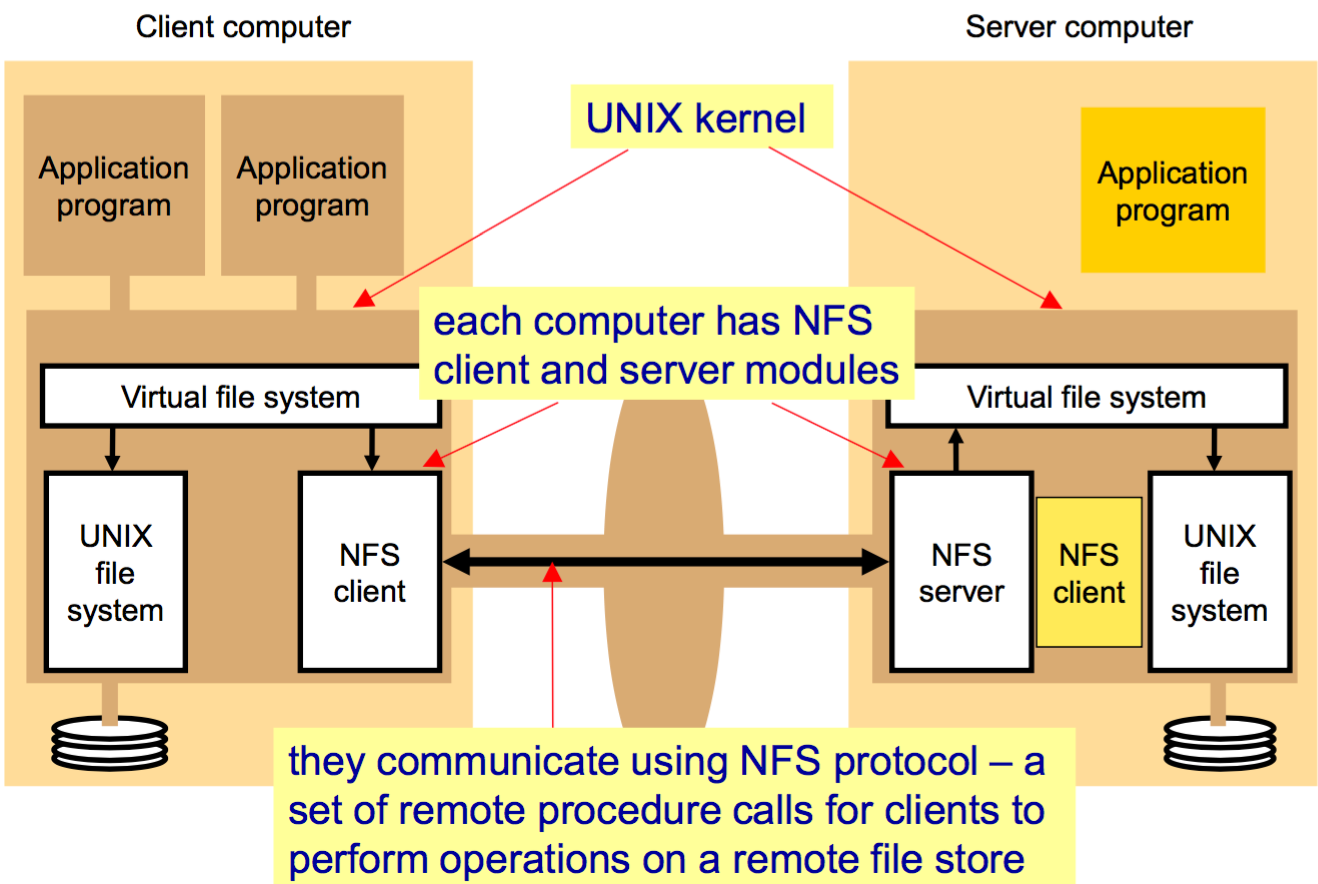
\includegraphics[width=8cm]{sun-file-system}
\end{center}

\noindent Each computer can act as both a client and a server.

\noindent File are accessed by file identifiers. File identifier is independent of the file name, created by the server hosting the file system and unique with respect to all files in the system. 

\subsection{Client-Server Communication}

\noindent NFS server operations are stateless and idempotent, so at-least-once invocation semantics can be used.\\

\noindent NFS client operations need to supply an interface suitable for use by conventional application programs. The interface emulates UNIX file system semantics. \\

\subsection{Mount Service}

\noindent File systems have to be exported by the server and be mounted by a client before they can be accessed by the client.\\

\noindent At the server, a mount service process runs at user level on each server. A file \verb|/etc/exports| contains the names of local file systems available for remote mounting and access list. \\

\noindent Client side use a modified UNIX mount command to request mounting, specifying remote host name, pathname of a directory in remote file system, and local name to be mounted. The command communicates with mount service process using PRC protocol. A table of mounted file systems is maintained at the client.\\

\noindent NFS does not enforce a single network-wide file name space. Clients can assign different local names to the same remote directory.\\

\noindent Pathnames are parsed, and their translation is performed in an iterative manner by clients. For example, if the root directory of a remote server is mounted, access to \verb|/bin/draw/readme| on the server requires three lookup request:
\begin{itemize}
    \item \verb|lookup(rootfh, "bin")| $\rightarrow$ \verb|bin| file handler
    \item \verb|lookup(binfh, "draw")| $\rightarrow$ \verb|draw| file handler
    \item \verb|lookup(drawfh, "readme")| $\rightarrow$ \verb|readme| file handler
\end{itemize}

\noindent To improve efficiency, we using caching to take advantage of reference locality. For example, if \verb|/bin/draw/install| is accessed soon after \verb|/bin/draw/readme| on the same server, only one lookup request to the server is needed.

\subsection{Client Caching}

\noindent NFS client caches file data at block level to reduce communication with server. However, writing operation by a client do not result in immediate updating of cached copies of the same file in other clients. To maintain cache consistency, clients are responsible for polling the server to check the currency of cached data they hold. \\

\noindent NFS provides a close approximation to one-copy semantics:
\begin{itemize}
    \item Each cache entry is tagged with two timestamps:
    \begin{enumerate}
        \item The last validation time of cache, $T_c$
        \item The last modified time of cached file at server $T_{\text{mclient}}$
    \end{enumerate}
    \item Entry is considered valid when $T-T_c < t$, where $t$ is a freshness interval and $T$ is currect time
    \item When client want to access a cached file:
    \begin{itemize}
        \item If $T-T_c<t$, read data from cache
        \item If $T-T_c\ge t$, get $T_{\text{mserver}}$ from server. If $T_{\text{mclient}}=T_{\text{mserver}}$, update $T_c$ and $T_{\text{mclient}}$ to current time. If $T_{\text{mclient}}<T_{\text{mserver}}$, send a new request to server to get new file.
    \end{itemize}
\end{itemize}

\subsection{Summary}

\noindent NFS achieves access transparency because application use the same file operations for both local and remote files.\\

\noindent NFS does not achieve location transparency because different clients can mount the same server directory to different local directories. 

\section{Andrew File System}

\noindent Andrew File System (AFS) are designed for scalability. AFS nodes are paritioned into two groups: (1) dedicated file servers and (2) a large number of clients. \\

\noindent Similar to NFS: 
\begin{itemize}
    \item Client can access to AFS files via normal UNIX file system operations.
    \item Venus clients and vice servers communicate using RPC
    \item Venus translates the pathnames into file identifiers using a step-by-step lookup
    \item File are accessed by file identifiers
\end{itemize}

\noindent Vice servers maintain a globally shared file name space. Clients have access to shared name space by means of a special local subdirectory \verb|/afs|. \\

\noindent Shared files are grouped into volumes for ease of replication.

\subsection{Server-side Replication}

\noindent Each file is contained in exactly one logical volumne and each logical volume may have several physical volumes. \\

\noindent Each logical volume is associated with a Replicated Volume Identifier (RVID, location and replication-independent) and each physical volume is associated with a Volume Identifier (VID, location-independent).\\

\noindent Each shared file is identified by a unique file identifier (RVID + file handle). \\

\noindent Consistency for AFS server-side replication is read-one, write-all. 

\subsection{Whole-file Serving and Caching}

\noindent Whole-file serving: entire files are transmitted to clients by AFS servers.\\

\noindent Whole-file caching: files transferred to a client are stored in a cache on local disk to satisfy future requests. When client close a file, the client transmits the updates to the server and retains the local copy.\\

\noindent AFS uses session update semantics to be more scalable. All other clients are able to see a modified file only after the file is closed by the client that modified it.\\

\noindent Callback mechanism is used to maintain cache consistency of client side. Vice server will issue a callback promise in \textit{valid} state to Venus client when the server sends a fresh file copy to client. When there is a update of the file at server side, the server will inform all clients with valid callback promise and remove these clients from its callback list. When a client receives a callback from the server, the client sets the callback promise to \textit{cancelled}.\\

\noindent However, if there is an update at server side before a client close a session / file, the callback has no effect on the file at currect session. If multiple clients write to a file concurrently, all update are silently lost except those of the last client closing the file. 

\subsection{Coda File System}

\noindent The main design goal of Coda file system is high availability. It allows clients to continue operation despite being disconnected from a server. Clients can use its locally cached copy of the files when disconnected from servers and reconcile later when the connection is established again. \\

\noindent To ensure client caches contain files that will be accessed during disconnection, we use hoarding technique, which fills the cache in advance with useful files:
\begin{itemize}
    \item We first ask user to specify useful files in a hoard database. Then, priorities for each file are computed using hoard database and information on recent file accesses.
    \item We fetch files in priority to reach equilibrium, when all cached files have higher priorities than uncached files, cache is full, all uncached files have zero priority, or cached files are up-to-date. 
    \item We do a hoard walk to periodically reorganize the cache to maintain equilibrium. 
\end{itemize}

\noindent There are 3 states of Coda client with respect to a volume: hoarding, emulation, and reintegration. 

\begin{center}
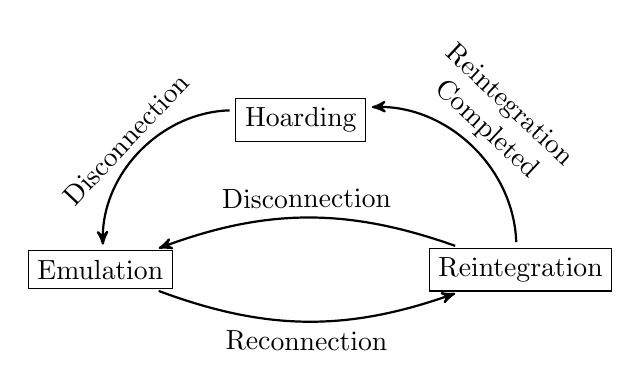
\begin{tikzpicture}[
node distance=1.5cm,
roundnode/.style={rectangle, draw=black, thin},
]
%Nodes
\node[roundnode](Hoarding){Hoarding};
\node[below=of Hoarding](dummy){};

\node[roundnode](Emulation)[left=of dummy]{Emulation};

\node[roundnode](Reintegration)[right=of dummy]{Reintegration};

\path[pil] (Reintegration) edge [bend right=45] node [pos=0.5, sloped, above, align=center] {Reintegration\\Completed} (Hoarding);
\path[pil] (Hoarding) edge [bend right=45] node [pos=0.5, sloped, above] {Disconnection} (Emulation);
\path[pil] (Emulation) edge [bend right=20] node [pos=0.5, sloped, below] {Reconnection} (Reintegration);
\path[pil] (Reintegration) edge [bend right=20] node [pos=0.5, sloped, above] {Disconnection} (Emulation);

\end{tikzpicture}
\end{center}

\noindent When the connection is established again, updates made to files during disconnection are transferred to the server. In case of conflicts, we can use automatic conflict resolution or manual intervention to resolve conflict. However, conflicts are rare because most files are written by only one user at a time. 

\end{multicols*}

\chapter{Peer-to-peer File Sharing Systems}
\begin{multicols*}{2}

\noindent All processes play similar roles and they interact cooperatively as peers to perform distributed computation. Every node provides some services that helps other nodes in the network to get services. \\

\noindent We will look at three unstructured P2P File Sharing, i.e. Napster, Gnutella, and KaZaA, and three structured DHT Systems, i.e. Distributed Hash Table Services, Consistent Hashing, and Chord.

\section{Napster}

\noindent Napster has a centralized directory server for centralized search, but file downloads are done in a distributed way. The centralized server has difficult time keeping up with increasing traffic.\\

\noindent All clients will upload file list and IP address to Napster centralized directory. Users will search for files using the centralized directory. When users found the file they want, they pings hosts that have the file to look for the best transfer rate for downloading.

\section{Gnutella}

\noindent Gnutella uses a decentralized method to search for files. Each application instance has the responsibility to store files, serve files, route queries and respond to queries. \\

\noindent However, Gnutella use flooding strategy to search for files, and reverse path forwarding is used for responses. The actual downloading is done by point-to-point TCP. As a result, each query can generate huge amount of traffic. Users can limit the number of hops to travel by setting the TTL field.\\

\noindent To establish connection, we first connect to a bootstrap node to get IP addresses of existing Gnutella nodes. Then, we send join messages to some existing Gnutella nodes.

\section{KaZaA}

\noindent KaZaA provides powerful file search and transfer service without server infrastructure using hierarchical architecture. Frequent uploaders can get priority in server queue. \\

\noindent Nodes that have more connection bandwidth and are more available are designated as supernodes. Each supernode acts as a mini-Napster hub, tracking the contents and IP addresses of its children. \\

\noindent Connection: A list of potential supernodes are included within the software. New peer goes through the list until it finds an operational supernode.\\

\noindent Metadata: When a node connects to a supernode, it uploads its metadata, i.e. file name, file size, content hash, and file description.\\

\noindent Query: Node first sends keyword query to supernode. If supernode cannot get enough number of matches, it forwards query to subset of supernodes. Query results contain the ContentHash of the wanted file and a list of nodes holding the file.\\

\noindent Download: If file is found in multiple nodes, user can download the files parallelly.

\section{Distributed Hash Table Services}

\noindent In Distributed Hash Table (DHT), we want to assign particular nodes to hold particular contents and arrange neighbour relationship between nodes in a restrictive structure to facilitate query routing.\\

\noindent We use hash function to map files to unique identifiers. Each node is responsible for the files that hash within its range, it must know the location of the files (indirect) or physically store the files (direct). \\

\noindent Query must be efficiently routed to the node whose range covers the file. This should be implemented in a fully distributed manner. \\

\noindent When nodes join / leave the system, we need bootstrap mechanism, repartition range space, and update routing information.

\section{Consistent Hashing}

\noindent We need to choose the range space of hash function as \emph{a circle of identifiers} from $0$ to $2^m -1$. $m$ must be large enought to avoid collision of two identifiers. \\

\noindent Each node is assigned the range space from the identifier of its counter-clockwise neighbour node on the identifier circle to its own identifier.\\

\noindent If each node maintains the identifier and IP address of its successor node, the complexity of routing information maintained at each node is $O(1)$ and the complexity of query routing is $O(N)$\\

\noindent If each node maintains the identifiers and IP addresses of all nodes, the complexity of routing information maintained at each node is $O(N)$ and the complexity of query routing is $O(1)$

\section{Chord}

\noindent Each node $n$ maintains identifiers and IP addresses of $m$ successors. The $i$-th entry in the finger table contains the first node that succeeds $n$ by at least $2^{i-1}$ on the identifier circle. \\

\noindent In routing, each node $n$ sends a query for key $k$ to the node in entry:

$$\lfloor log_2(k-n) \rfloor + 1$$

\noindent The complexity of routing information maintained at each node is $O(log(N))$ and the complexity of query routing is $O(log(N))$\\

\noindent Joining and leaving process work like insertion and deletion in a double-linked list. When joining, the node need to copy the location information of all keys within its range from its sucessor, and then need to build the finger table and update all current finger tables. The complexity is $O(log^2(N))$.


\end{multicols*}

\chapter{Name Services}
\begin{multicols*}{2}

\noindent Names identify resources in a \emph{location-independent} fashion. Addresses identify resources in a \emph{location-dependent} fashion.\\

\noindent Name service does translation between names and addresses. Name resolution is the conversion process from names to addresses. 

\noindent Main requirements of name services:
\begin{itemize}
  \item Scalability: to handle arbitrary number of names and to serve an arbitrary number of administrative organizations over long lifetime
  \item Reliability: name services should not fail frequently
  \item Performance: name resolution should have short response time
\end{itemize}

\noindent Name space is the collection of all valid names. Name space requires a syntatic definition. Name space can have hierarchical structure or flat structure, but hierarchical name space has better scalability than flat name space.

\section{Name Resolution Process}

\noindent Physically, the resolution process may involve more than on name server because the mapping may not be available at every name server.\\

\noindent Method 1: Iterative Client-controller Navigation. A client iteratively contacts a group of name servers to resolve a name. However, this method has high communication cost if name servers are located far away.\\

\noindent Method 2: Non-recursive Server-controller Navigation. A name server coordinates the name resolution process iteratively or multicast on behalf of a client.\\

\noindent Method 3: Recursive Server-controller Navigation. If a name server does not have the name mapping, it contact another name server, and this procedure continues recursively until the anem is resolved. The caching results is more effective, but it put higher performance demand on each name server.

\section{Domain Name System}

\noindent To meet requirements of name services, DNS uses:
\begin{itemize}
  \item Scalability: hierarchical name space
  \item Reliability: use replication
  \item Performance: use caching
\end{itemize}

\subsection{Hierarchical Name Space}

\begin{center}
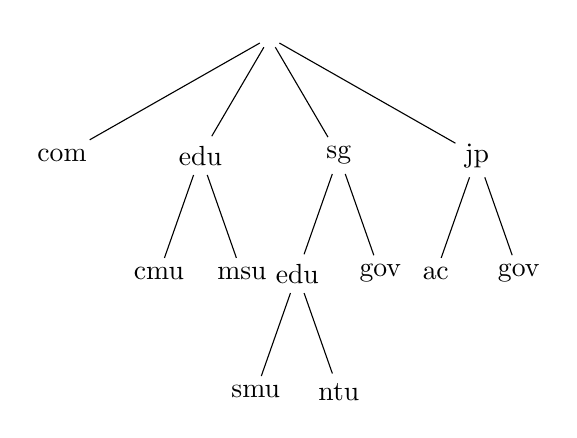
\begin{tikzpicture}[
recnode/.style={rectangle, draw=white, thin},
level 1/.style={sibling distance=5em},
level 2/.style={sibling distance=3em},
]
%Nodes
\node[recnode,draw](Top){}
    child {node[recnode,draw](com){com} edge from parent[-]}
    child {node[recnode,draw](edu){edu} edge from parent[-]
      child {node[recnode,draw](cmu){cmu} edge from parent[-]}
      child {node[recnode,draw](msu){msu} edge from parent[-]}
    }
    child {node[recnode,draw](sg){sg} edge from parent[-]
      child {node[recnode,draw](edu2){edu} edge from parent[-]
        child {node[recnode,draw](smu){smu} edge from parent[-]}
        child {node[recnode,draw](ntu){ntu} edge from parent[-]}
      }
      child {node[recnode,draw](gov){gov} edge from parent[-]}
    }
    child {node[recnode,draw](jp){jp} edge from parent[-]
      child {node[recnode,draw](ac){ac} edge from parent[-]}
      child {node[recnode,draw](gov2){gov} edge from parent[-]}
    }
;
\end{tikzpicture}
\end{center}

\noindent DNS uses a decentralized design, i.e no single server is responsible for all names. The entire name spaces is partitioned among a large group of name servers. Each server holds authoritative mappings for the names in one or more domains. \\

\noindent Each mapping contains domain name, time-to-live, class, type and value. The information held in DNS servers are:
\begin{itemize}
  \item Mappings between names and IP addresses for the local domain
  \item Names and addresses of all name servers in local domain, sub-domains, and root name servers
\end{itemize}

\noindent Type of mapping:
\begin{itemize}
  \item A-type record maps a computer name to its IP address
  \item CNAME-type record maps an alias to its canonical name
  \item NS-type record specifies authoritative name servers. Each NS-record is accompanied by an A-type record.
  \item MX-type record gives preferences and domain names of mail hosts
\end{itemize}

\subsection{Replication for Reliability}

\noindent Authoritative mappings of each domain must be held by at least two name servers, i.e. the primary server and secondary servers. Secondary servers periodically check with the primary server to see whether their stored mappings are up-to-date. \\

\noindent DNS uses a simple request-reply protocol between clients and name servers based on UDP. DNS primarily uses a combination of iterative client-controlled navigation and non-recursive server- controlled navigation. 

\subsection{Caching for Performance Improvement}

\noindent Results of name resolution may be cached by clients and name servers. Clients and name servers always consult their caches before sending queries to other servers for name resolution. \\

\noindent However, caching introduces inconsistency problem. Query answers returned from cached mappings may be out-of-date. The consistency problem can be addressed by timeouts (time-to-live values).

\end{multicols*}

\chapter{Time and Global States}
\begin{multicols*}{2}

\noindent Although one of the property of distributed system is no globally shared clock, many distributed applications still depend on timing.

\section{Synchronizing Physical Clock}

\noindent Computers have their own physical clocks that deviate from one another. Universal Coordinated Time (UTC) is commonly used reference clock.\\

\noindent \emph{Clock drift}: clock count time at different rates.\\

\noindent \emph{Drift rate}: the change in offset between a clock and a perfect reference clock per unit of time measured by the reference clock.

\subsection{Cristian's Method}

\noindent The algorithm:

\begin{enumerate}
  \item $A$ requests the time of $B$
  \item $B$ replies with the time value $t$
  \item $A$ records the total RTT, $T_{\text{round}}=t_2 - t_1$
  \item $A$ sets its clock to $t + T_{\text{round}} / 2$
\end{enumerate}

\noindent To calculate the accuracy of Cristian's Method, we need to consider 2 cases:
\begin{enumerate}
  \item When the transmission time of reply message approaches $0$, $B$'s clock reading is $t$.
  \item When the transmission time of reply message approaches $T_{\text{round}}$, $B$'s clock reading is $t+ T_{\text{round}}$.
\end{enumerate}

\noindent When $A$ receives the reply, the time reading on $B$ should be in $[t,t+ T_{\text{round}}]$. $A$ is accurate within bound $T_{\text{round}} / 2$

\subsection{Berkeley Algorithm}

\noindent The algorithm:
\begin{enumerate}
  \item Master periodically polls slaves
  \item Slaves send their clock readings back
  \item Master evaluates the local times of slaves by observing the RTT
  \item Master averages the values obtained and its own clock reading
  \item Master sends the amount of adjustment to each slave
\end{enumerate}

\noindent We use average clock reading because it cancels out individual clocks' tendencies to run fast or slow. 

\subsection{Network Time Protocol}

\noindent Cristian's method and Berkeley algorithm use centralized design. Network Time Protocol (NTP) is used to distribute time information over the Internet. \\

\noindent NTP has a network of servers structured hierarchically into a synchronization subnet. This setup is fault-tolerance because servers can reconfigure themselves if someone becomes unreachable. 

\subsubsection{Analysis of Accuracy}
\begin{center}
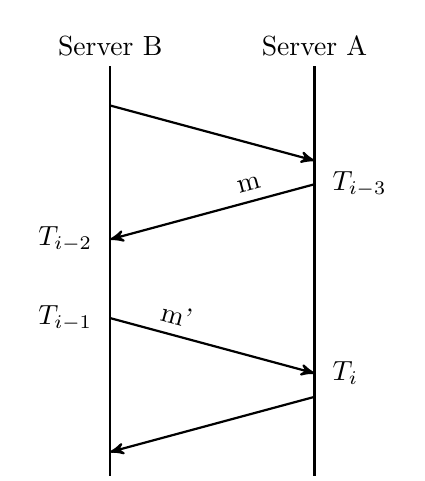
\begin{tikzpicture}[>=stealth',thick,
commentl/.style={text width=0.7cm, align=right},
commentr/.style={commentl, align=left},]
\node[] (init) {Server B};
\node[right=1cm of init] (recv) {Server A};

\draw[->] ([yshift=-.5cm]init.south) coordinate (send1) -- ([yshift=-.7cm]send1-|recv) coordinate (send1done) node[pos=.3, above, sloped] {};

\draw[->] ([yshift=-.3cm]send1done) coordinate (reply1) -- ([yshift=-.7cm]reply1-|init) coordinate (reply1done) node[pos=.3, above, sloped] {m};

\draw[->] ([yshift=-1cm]reply1done) coordinate (send2) -- ([yshift=-.7cm]send2-|recv) coordinate (send2done) node[pos=.3, above, sloped] {m'};

\draw[->] ([yshift=-.3cm]send2done) coordinate (reply2) -- ([yshift=-.7cm]reply2-|init) coordinate (reply2done) node[pos=.3, above, sloped] {};

\draw[thick, shorten >=-1cm] (init) -- (init|-reply2);
\draw[thick, shorten >=-1cm] (recv) -- (recv|-reply2);

\node[commentr, right =1mm of reply1] {$T_{i-3}$};
\node[left = 1mm of reply1done.west, commentl]{$T_{i-2}$};
\node[left = 1mm of send2.west, commentl]{$T_{i-1}$};
\node[commentr, right =1mm of send2done] {$T_{i}$};
\end{tikzpicture}
\end{center}

\noindent Time between sending of $m$ and receipt of $m'$ is $$T_i - T_{i-3}$$
\noindent Time between receipt of $m$ and sending of $m'$ is $$T_{i-1} - T_{i-2}$$
\noindent The total transmission time of $m$ and $m'$ is $$(T_i - T_{i-3}) - (T_{i-1} - T_{i-2})$$
\noindent The transmission time of $m'$ is $$[0,(T_i - T_{i-3}) - (T_{i-1} - T_{i-2})]$$
\noindent If transmission time of $m'$ approaches $0$, when A receives $m'$ B clock reading is $$T_{i-1}$$
\noindent If transmission time of $m'$ approaches $(T_i - T_{i-3}) - (T_{i-1} - T_{i-2})$, when A receives $m'$ B clock reading is $$T_{i-1} + (T_i - T_{i-3}) - (T_{i-1} - T_{i-2}) = T_i - T_{i-3} + T_{i-2}$$
\noindent If A want to synchronize with B as accurately as possible, A should set its clock to $$\frac{1}{2}(T_{i-1} + (T_i - T_{i-3} + T_{i-2})$$

\noindent The accuracy is $$\pm \frac{1}{2}(T_{i-1} - (T_i - T_{i-3} + T_{i-2})$$

\section{Causal Ordering and Logical Clocks}

\noindent We refer the state of process $p_i$ and as $s_i$, and there are $i=1\ldots N$ number of processes.\\

\noindent Process takes a series of actions, i.e. sending a message, receiving a message, or transforms the state of the process.\\

\noindent An event is the occurrence of a single action.

\subsection{Causal Ordering}

\noindent Events can be ordered based on cause-and-effect. Event within a single process $p_i$ can be placed in a unique total ordering. The event of sending the message occurs before the event of receiving the message. 

\begin{center}
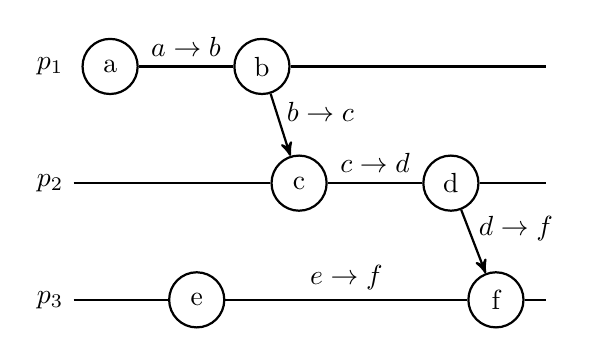
\begin{tikzpicture}[>=stealth',thick,
roundnode/.style={circle, draw=black, thick, minimum size=0.7cm},
]
\node[] (p1) {$p_1$};
\node[below=1cm of p1] (p2) {$p_2$};
\node[below=1cm of p2] (p3) {$p_3$};

\node[roundnode](a)[right = 1mm of p1.east]{a};
\node[roundnode](b)[right = 12mm of a.east]{b};

\node[roundnode](c)[right = 25mm of p2.east]{c};
\node[roundnode](d)[right = 12mm of c.east]{d};

\node[roundnode](e)[right = 12mm of p3.east]{e};
\node[roundnode](f)[right = 50mm of p3.east]{f};

\node[right = 60mm of p1](d1){};
\node[right = 60mm of p2](d2){};
\node[right = 60mm of p3](d3){};

\draw[-] (a) -- (b) node [pos=0.5, above, align=center] {$a\rightarrow b$};
\draw[->] (b) -- (c) node [pos=0.3, right, align=center] {$b\rightarrow c$};
\draw[-] (c) -- (d) node [pos=0.5, above, align=center] {$c\rightarrow d$};
\draw[->] (d) -- (f) node [pos=0.3, right, align=center] {$d\rightarrow f$};
\draw[-] (e) -- (f) node [pos=0.5, above, align=center] {$e\rightarrow f$};
% Dummy 
\draw[-] (b) -- (d1);
\draw[-] (p2) -- (c);
\draw[-] (d) -- (d2);
\draw[-] (p3) -- (e);
\draw[-] (f) -- (d3);

\end{tikzpicture}
\end{center}

\noindent From the figure above, we can deduce that $a$ happens before $f$, $a\rightarrow f$, and $a$ is parallel to $e$, $e\|e$ 

\subsection{Lamport's Logical Clocks}

\noindent Logical clock is a monotonically increasing software counter whose value bears no particular relationship with real time. 

\begin{center}
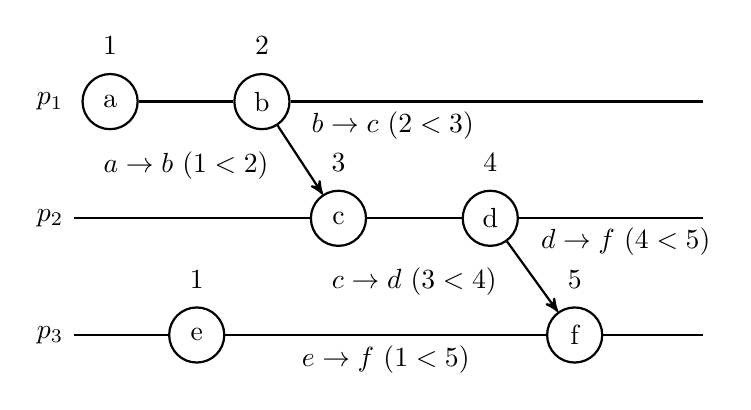
\begin{tikzpicture}[>=stealth',thick,
roundnode/.style={circle, draw=black, thick, minimum size=0.7cm},
]
\node[] (p1) {$p_1$};
\node[below=1cm of p1] (p2) {$p_2$};
\node[below=1cm of p2] (p3) {$p_3$};

\node[roundnode](a)[right = 1mm of p1.east]{a};
\node[roundnode](b)[right = 12mm of a.east]{b};

\node[roundnode](c)[right = 30mm of p2.east]{c};
\node[roundnode](d)[right = 12mm of c.east]{d};

\node[roundnode](e)[right = 12mm of p3.east]{e};
\node[roundnode](f)[right = 60mm of p3.east]{f};

\node[right = 80mm of p1](d1){};
\node[right = 80mm of p2](d2){};
\node[right = 80mm of p3](d3){};

\draw[-] (a) -- (b) node [pos=0.5, below = 5mm, align=center] {$a\rightarrow b\ (1<2)$};
\draw[->] (b) -- (c) node [pos=0, right = 3mm, align=center] {$b\rightarrow c\ (2<3)$};
\draw[-] (c) -- (d) node [pos=0.5, below = 5mm, align=center] {$c\rightarrow d\ (3<4)$};
\draw[->] (d) -- (f) node [pos=0, right = 3mm, align=center] {$d\rightarrow f\ (4<5)$};
\draw[-] (e) -- (f) node [pos=0.5, below, align=center] {$e\rightarrow f\ (1<5)$};

% Dummy 
\draw[-] (b) -- (d1);
\draw[-] (p2) -- (c);
\draw[-] (d) -- (d2);
\draw[-] (p3) -- (e);
\draw[-] (f) -- (d3);

% Label
\node[above=1mm of a](labela){1};
\node[above=1mm of b](labelb){2};
\node[above=1mm of c](labelc){3};
\node[above=1mm of d](labeld){4};
\node[above=1mm of e](labele){1};
\node[above=1mm of f](labelf){5};

\end{tikzpicture}
\end{center}

\noindent From the diagram above, since $a\rightarrow f$, so $L(a)<L(e')$. This is always true, but the converse is not. Specifically, if $L(e)<L(e')$, we cannot infer that $e\rightarrow e'$.

\subsection{Vector Clocks}

\noindent A vector clock for $N$ processes is an array of $N$ integers. Each process has its own vector clock. 

\begin{center}
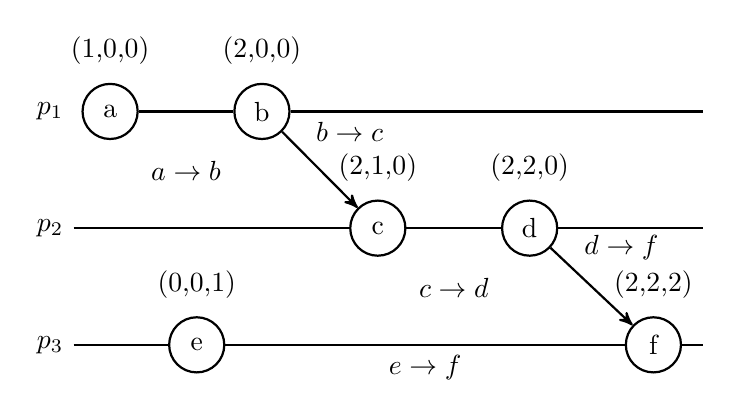
\begin{tikzpicture}[>=stealth',thick,
roundnode/.style={circle, draw=black, thick, minimum size=0.7cm},
]
\node[] (p1) {$p_1$};
\node[below=1cm of p1] (p2) {$p_2$};
\node[below=1cm of p2] (p3) {$p_3$};

\node[roundnode](a)[right = 1mm of p1.east]{a};
\node[roundnode](b)[right = 12mm of a.east]{b};

\node[roundnode](c)[right = 35mm of p2.east]{c};
\node[roundnode](d)[right = 12mm of c.east]{d};

\node[roundnode](e)[right = 12mm of p3.east]{e};
\node[roundnode](f)[right = 70mm of p3.east]{f};

\node[right = 80mm of p1](d1){};
\node[right = 80mm of p2](d2){};
\node[right = 80mm of p3](d3){};

\draw[-] (a) -- (b) node [pos=0.5, below = 5mm, align=center] {$a\rightarrow b$};
\draw[->] (b) -- (c) node [pos=0, right = 3mm, align=center] {$b\rightarrow c$};
\draw[-] (c) -- (d) node [pos=0.5, below = 5mm, align=center] {$c\rightarrow d$};
\draw[->] (d) -- (f) node [pos=0, right = 3mm, align=center] {$d\rightarrow f$};
\draw[-] (e) -- (f) node [pos=0.5, below, align=center] {$e\rightarrow f$};

% Dummy 
\draw[-] (b) -- (d1);
\draw[-] (p2) -- (c);
\draw[-] (d) -- (d2);
\draw[-] (p3) -- (e);
\draw[-] (f) -- (d3);

% Label
\node[above=1mm of a](labela){(1,0,0)};
\node[above=1mm of b](labelb){(2,0,0)};
\node[above=1mm of c](labelc){(2,1,0)};
\node[above=1mm of d](labeld){(2,2,0)};
\node[above=1mm of e](labele){(0,0,1)};
\node[above=1mm of f](labelf){(2,2,2)};

\end{tikzpicture}
\end{center}

\noindent If $e\rightarrow e'$, then $V(e)\rightarrow V(e')$. 

\noindent If $V(e)\rightarrow V(e')$, then $e\rightarrow e'$. 

\noindent If $e\|e'$, then neither $V(e)\le V(e')$ nor $V(e')\le V(e)$

\section{Global States}

\noindent In many situations, we need to find out whether a particular property is true when a distributed system executes. We want to assemble a meaningful global state from local states recorded by different process at different real times.\\

\noindent The state of process $p_i$ is the state immediately after its $k$-th event occurs. Global state is a set of states of all processes.

\subsection{Consistent Cut} \label{section:consistent-cut}

\noindent A consistent cut is a cut $C$, such that for all events $\forall e\in C$, $\exists f \in C, f\rightarrow e$. Otherwise, the cut is unconsistent. 

\tiny
\begin{center}
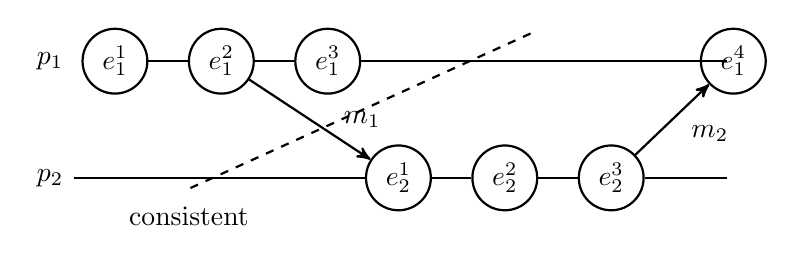
\begin{tikzpicture}[>=stealth',thick,
roundnode/.style={circle, draw=black, thick, minimum size=0.3cm},
]

\node[] (p1) {$p_1$};
\node[below=1cm of p1] (p2) {$p_2$};

\node[roundnode](e11)[right = 1mm of p1.east]{$e_1^1$};
\node[roundnode](e12)[right = 5mm of e11.east]{$e_1^2$};
\node[roundnode](e13)[right = 5mm of e12.east]{$e_1^3$};
\node[roundnode](e14)[right = 43mm of e13.east]{$e_1^4$};

\node[roundnode](e21)[right = 37mm of p2.east]{$e_2^1$};
\node[roundnode](e22)[right = 5mm of e21.east]{$e_2^2$};
\node[roundnode](e23)[right = 5mm of e22.east]{$e_2^3$};

\node[right = 83mm of p1](d1){};
\node[right = 83mm of p2](d2){};

\draw[-] (e11) -- (e12);
\draw[-] (e12) -- (e13);
\draw[-] (e13) -- (e14);

\draw[->] (e12) -- (e21) node [pos=0.5, right = 3mm, align=center] {$m_1$};
\draw[-] (e21) -- (e22);
\draw[-] (e22) -- (e23);
\draw[->] (e23) -- (e14) node [pos=0.3, right = 3mm, align=center] {$m_2$};

% Dummy 
\draw[-] (p2) -- (e21);
\draw[-] (e14) -- (d1);
\draw[-] (e23) -- (d2);

\draw[dashed] 
  ([yshift=10pt]$ (e13)!0.5!(e14) $ ) -- 
  ([yshift=-25pt]$ (e13)!0.5!(p2) $ ) node [below = 1mm] {consistent};

\end{tikzpicture}
\end{center}
\normalsize

\subsection{Recording a Snapshot}

\noindent To record a snapshot, we need to record the states of all processes and the state of communication channels.  

\subsubsection{Chandy and Lamport Algorithm}

\noindent The algorithm uses a marker messages to prompt the receiver to save its own local state and determine which messages to include in the channel state.

\noindent The algorithm:

\begin{itemize}
  \item Any process may initiate a snapshot recording at any time
  \item Each non-initiating process records its proces state on receiving the first marker message
  \item If $p_j$ is the initiating process, $p_j$ initiates the messages arriving on channel $c_{i\rightarrow j}$ between $p_j$ initiates the snapshot recording and receives the marker message from $p_i$
  \item If $p_j$ is non-initiating process and $c_{i\rightarrow j}$ is the channel through which $p_j$ receives its first marker message, $c_{i\rightarrow j}$ state is recorded as an empty set
  \item If $p_j$ is non-initiating process and $c_{i\rightarrow j}$ is not the channel through which $p_j$ receives its first marker message, $p_j$ records the message arriving on channel $c_{i\rightarrow j}$ between $p_j$ receives the first marker message and the marker message from $p_i$
  \item Each process completes all recording activities when it has received a marker message from all other processes. Then, it may send the recorded states (local process state + channel states) to the initiating process.
\end{itemize}

\section{Distributed Debugging}

\noindent We want to establish what occurred during the execution of a distributed system and to check whether they are correct. 

\subsection{Lattice of Consistent Global States}

\noindent Refering to the figure in section \ref{section:consistent-cut}, we will get the following lattice of consistent global states. The lattice is constructed by listing all consistent global states starting from the initial state and advance the global state by one event at a time. 

\begin{center}
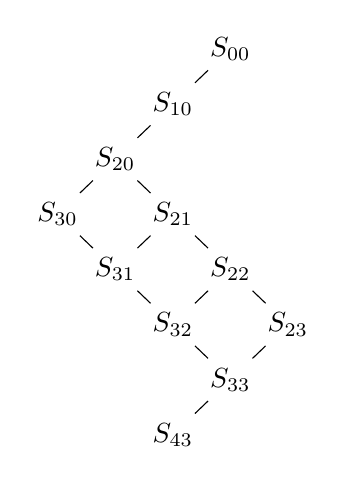
\begin{tikzpicture}[
recnode/.style={rectangle, draw=white, thin},
level distance=0.7cm,
level 1/.style={sibling distance=0.7cm},
level 2/.style={sibling distance=0.7cm},
level 3/.style={sibling distance=0.7cm},
level 4/.style={sibling distance=0.7cm},
level 5/.style={sibling distance=0.7cm},
level 6/.style={sibling distance=0.7cm},
level 7/.style={sibling distance=0.7cm},
level 8/.style={sibling distance=0.7cm},
]
%Nodes
\node[recnode,draw](s00){$S_{00}$}
  child[left] {node[recnode,draw](s10){$S_{10}$} edge from parent[-]
    child[left] {node[recnode,draw](s20){$S_{20}$} edge from parent[-]
      child[left] {node[recnode,draw](s30){$S_{30}$} edge from parent[-]}
      child[right] {node[recnode,draw](s21){$S_{21}$} edge from parent[-]
        child[left] {node[recnode,draw](s31){$S_{31}$} edge from parent[-]}
        child[right] {node[recnode,draw](s22){$S_{22}$} edge from parent[-]
          child[left] {node[recnode,draw](s32){$S_{32}$} edge from parent[-]}
          child[right] {node[recnode,draw](s23){$S_{23}$} edge from parent[-]
            child[left] {node[recnode,draw](s33){$S_{33}$} edge from parent[-]
              child[left] {node[recnode,draw](s43){$S_{43}$} edge from parent[-]}
              child[missing] {node[recnode,draw](d){} edge from parent[-]}
            }
            child[missing] {node[recnode,draw](d){} edge from parent[-]}
          }
        }
      }
    }
    child[missing] {node[recnode,draw](d){} edge from parent[-]}
  }
  child[missing] {node[recnode,draw](d){} edge from parent[-]}
;

\draw (s31) -- (s30);
\draw (s32) -- (s31);
\draw (s33) -- (s32);
\end{tikzpicture}
\end{center}

\noindent Each path from top-level state to the bottom level state in the lattice represents an ordering of all events that are consistent with causal ordering. Without global time, we cannot tell which one is the actual execution of the system among all possible executions.\\

\noindent In general, $<s_1^{c_i}, s_2^{c_j},\ldots,s_N^{c_N}>$ is a consistent global state if $V(e_i^{c_i})[i] \ge V(e_j^{c_j})[i]$ for any $i$ and $j$. \\

\noindent If there are only two processes, $S_{ij} = <s_1^{i}, s_2^{j}>$ is a consistent global state if $V(e_1^{i})[1] \ge V(e_2^{j})[1]$ and $V(e_2^{j}[2]) \ge V(e_1^{i})[2]$\\

\noindent To check whether a constraint is broken during execution, we need to evaluate whether each global state satisfies the constraint:
\begin{itemize}
  \item If all states satisfy the constraint, the constraint cannot be broken in the execution
  \item If there exists a state not satisfying the constraint, the constraint is possibly broken in the execution
  \item If every path from top to bottom passes through at least one state that does not satisfy the constraint, the constraint must be broken in the execution
\end{itemize}

\end{multicols*}

\chapter{Coordination and Agreement}
\begin{multicols*}{2}

\noindent Problems and issues in coordination and agreement:
\begin{itemize}
  \item Mutual exclusion: for processes to coordinate their accesses to shared resources
  \item Election: for processes to agree on a coordinator
  \item Consensus: for processes to agree on some value
\end{itemize}

\section{Distributed Mutual Exclusion}

\noindent Objective: to prevent interference when a set of processes access shared resources that require exclusive use.\\

\noindent Requirements for Mutual Exclusion:
\begin{enumerate}
  \item Safety: at most one process may execute in the critical section at a time
  \item Liveness: requests to enter and exit the critical section eventually succeed, no deadlock and starvation. 
\end{enumerate}

\subsection{Central Server Algorithm}

\noindent Token: permission to enter the critical section\\

\noindent To enter critical section, a process sends a request to the server and awaits a reply from it. If no other process has the token, the server replies immediately and granting the token. If there is another process has the token, the server queues the request. The process enters the critical section once it receives the token.\\

\noindent To exit a critical section, a process sends the token back to the server. The server will get the next process from the queue and grat the token.\\

\noindent The algorithm satisfies safety and liveness requirements, but the server is a single point of failure and can become a performance bottleneck. \\

\noindent Performance:

\begin{enumerate}
  \item Bandwidth consumption: entering critical section takes two message (request and grant), existing critical section takes one message (release)
  \item Client delay: Entering critical section delays the process by two message transmissions
  \item Synchronization delay: two message transmissions (release message to server and grant message to next process)
\end{enumerate}

\subsection{Ring-based Algorithm}

\noindent The algorithm:
\begin{itemize}
  \item A token is circulated in clockwise direction around the ring.
  \item On receiving token, if the process 
  \begin{itemize}
    \item does not require to enter critical section, it forwards the token
    \item does require to enter critical section, it retains the token and enters. The process sends the token to neigbour to exit critical section. 
  \end{itemize}
\end{itemize}

\noindent Performance:

\begin{itemize}
  \item Bandwidth consumption: if every process constantly wants to enter a critical section, each token pass results in one entry and exit.
  \item Client delay: between $0$ to $N$ message transmissions
  \item Synchronization delay: between $1$ and $N$ message transmissions
\end{itemize}

\subsection{Ricart and Agrawala Algorithm}

\noindent This algorithm requires a total ordering of all events. Each process is in either \verb|RELEASED|, \verb|WANTED|, or \verb|HELD| states.\\

\noindent The algorithm:
\begin{itemize}
  \item To enter critical section, a process change to \verb|WANTED| state and send request messages to all other processes. The process can enter critical section (\verb|HELD| state) only when all other processes have replied to the requests.
  \item When a process receives a request message, if the receiver is in \verb|HELD| state, it queue the request. If the receiver is in \verb|WANTED| state, it compares the timestamp of the request with its own request. If the request has smaller timestamp, reply. Else, queue the request.
  \item When the process exits critical section, change to \verb|RELEASED| state and reply to all queued requests.
\end{itemize}

\noindent Performance:

\begin{itemize}
  \item Bandwidth consumption: Entering critical section takes $N-1$ requests and $N-1$ replies.
  \item Client delay: entering critical section delays the process by 2 message transmission if all requests are sent simultaneously
  \item Synchronization delay: 1 message transmission
\end{itemize}

\section{Election}

\noindent Objective: to choose unique process (coordinator) to play a particular role.\\

\noindent Different processes may call elections concurrently, so we need to ensure a unique coordinator is elected. More processes may fail during election, so we need to ensure that non-crashed process is elected eventually.\\

\noindent We assume that each process has a unique identifier, and we require the coordinator with the largest identifier to be chosen.\\

\noindent Turnaround time: the number of serialized message transmission times between the initiation and termination of an election. 

\subsection{Ring-based Algorithm}

\noindent Arrage processes in a logical ring. A process is participant if it engaged in some elections, otherwise, it is non-participant.\\

\noindent The algorithm:
\begin{itemize}
  \item A process initiate an election by marking itself as participant, placing its identifier in the election message and send it to its neigbour.
  \item When a process receives election message, it compares the identifier in the message with its identifier.
  \begin{itemize}
    \item If arrived identifier is greater, forward the message
    \item If arrived identifier is smaller and the receiver is non-participant, substitude with own identifier and forward the message
    \item If arrived identifier is smaller and the receiver is participant, drop the message
    \item Once the process forwards the message, it marks itself as participant
    \item If the arrived identifier is equal, the process become coordinator. It marks itself as non-participant and sends elected message to neighbour. All other processes will marks themselve as non-participant, records the coordinator, and forwards the message.
  \end{itemize}
\end{itemize}

\noindent Performance:
\begin{itemize}
  \item Bandwidth consumption: when the anti-clockwise neighbour has the largest identifier, it takes $N-1$ messages to reach the neigbour, then $N$ more messages to complete the circuit, then $N$ elected messages. In total, we need $3N-1$ messages
  \item Turnaround time: $3N-1$ messages
\end{itemize}

\subsection{Bully Algorithm}

\noindent This algorithm allows process to crash during an election. It assumes synchronous system and uses timeouts to detect process crash. If no response arrives within time $T=2T_{\text{trans}} + T_{\text{process}}$, then intended recipient must have crashed.\\

\noindent We assume that each process knows which processes have larger identifiers and it can communicate with all such processes.\\

\noindent The algorithm:

\begin{itemize}
  \item Any process that detects the coordinator crashes can start an election. When the process begins an election:
  \begin{itemize}
    \item The process sends election messages to all processes with larger identifiers.
    \item If no answer message responds within time T, the process wins the election and becomes coordinator. The process announces the result of election by seding coordinator messages to all processes.
    \item If some process responds within answer message, the process waits for coordinator message to arrive from new coordinator
  \end{itemize}
  \item When a process receives an election message, the process sends back answer message and starts an election
  \item If a crashed process comes back up, and it knows that it has the largest identifier, it announces that it is coordinator by sending coordinator messages.
\end{itemize}

\noindent Performance:
\begin{itemize}
  \item Bandwidth consumption: 
  \begin{itemize}
    \item Best case: the process with the second largest identifier detects the crash, $1$ election message and $N-2$ coordinator messages.
    \item Worst case: the process with the smallest identifier detects the crash, we need $O(N^2)$ messages.
  \end{itemize}
  \item Turnaround time: Best case: $T$ + 1 message transmission
\end{itemize}

\section{Consensus Problem}

\noindent Objectives: for processes to agree on a value even in the presence of failtures after one or more processes have proposed the value.\\

\noindent Requirements of Consensus Problem:
\begin{itemize}
  \item Termination: each correct process sets its decision variable eventually
  \item Agreement: the decision values of all correct processes are the same
  \item Integrity: if the correct processes all proposed the same value, then any correct process in the decided state has chosen that value
\end{itemize}

\subsection{Consensus in Synchronous System}

\noindent We assume that up to $f$ of the $N$ processes may crash.\\

\noindent In the absence of process crash, each process $p_i$ multicasts its proposed value $v_i$ to all other process and waits until it has collected all $N$ values and then evaluates a function to set its decision variable.\\

\noindent When processes crash, the processes may not actually send values to all other processes. So not all processes receive the same set of values.\\

\noindent To solve the problem, we run the algorithm for $f+1$ rounds. At the end of the last round, all correct processes that survice must have received the same set of values. 

\subsection{Consensus in Asynchronous System}

\noindent No algorithm can guarantee to reach consensus in asynchronous systems even if there is only one faulty process

\end{multicols*}

\chapter{Replication and Consistency}
\begin{multicols*}{2}

\noindent Data replication means maintaining copies of data at multiple computers to improve performance, scalability, reliability and fault-tolerance. However, we need to pay the price of consistency of replicas.

\section{Data-Centric Consistency Models}

\noindent To provide a system wide consistent view of data objets when concurrent processes simultaneously update data objects.

\noindent Target scenario: concurrent processes may simultaneously update data objects.

\subsection{Strict Consistency}

\noindent Any read operation on a data object returns a value corresponding to the result of the most recent write operation on the object. All wirtes are instaneously visible to all clients. \\

\noindent In the absence of a global clock in distributed system, it is difficult to assign a unique timestamp to each operation that corresponds to actual global time. It is also difficult to define precisely which write operation is the most recent. 

\subsection{Sequential Consistency}

\noindent The result of any execution is the same as if the operations by all clients were executed in some sequential order. The operation of each individual client appear in this sequence in the order specified by its program. 

\subsection{Causal Consistency}

\noindent Causal consistency makes distinction between events that are potentially causally related and those that are not. A read is causally related to the write that provided the data the read got.\\

\noindent Writes that are potentially causally related must be seen by all clients in the same order. Concurrent writes may be seen in different orders by different clients. 

\subsection{FIFO Consistency}

\noindent Writes done by a single client are seen by other clients in the order in which they were issued. Writes from different clients may be seen in different orders by different clients. 

\section{Consistency Protocols}

\noindent A consistency protocol describes an actual implementation of a specific consistency model.

\subsection{Primary-Based Protocols}

\noindent For each data object, one replica is designated as the primary replica and the remaining replicas are called backups / slaves. 

\subsubsection{Remote-Write Protocol}

\noindent Implementation of sequential consistency. The algorithm:

\begin{itemize}
  \item Write operations are forwarded to the primary replica. The primary replica performs the update and then forwards the update to the backup replicas.
  \item Each backup replica performs the update as well and sends an acknowledgement back to the primary replica
  \item Finally, the primary replica sends an acknowledgement back to the initiating client.
\end{itemize}

\noindent Write operations are blocking, read operations can be carried out at any replica. 

\subsubsection{Local-Write Protocol}

\noindent The algorithm:
\begin{itemize}
  \item The primary replica is migrated to the replica that receive client request. 
  \item As soon as the primary replica has updated its local copy, it returns an acknowledgement to the client
  \item Then, the primary replica tells the backup replicas to perform the update
\end{itemize}

\noindent Advantage: Multiple successive write operations can be carried out locally.

\subsection{Active Replication}

\noindent In active replication, all replicas play the same role and write operations are carried out at all replicas. Operations are sent to all replicas via totally ordered multicast. All replicas start in the same state and perform the same operations in the same order. \\

\noindent Write operations are blocking, and read operation can be carried out at any replica. \\

\noindent Active replication achieves sequential consistency. It can tolerate up to $f$ byzantine failture using $2f+1$ replicas.

\subsection{Gifford’s Quorum-Based Protocol}

\noindent A network partition separates a group of replicas into two or more subgroups in such a way that replicas of one subgroup can communicate with one another, but replicas of different subgroups cannot communicate with one another. \\

\noindent A quorum is a subgroup of replicas whose size gives it the right to perform operations.\\

\noindent In this protocol, update operation may be performed by one subset of replicas only. When a replica is updated, its version number is changed accordingly. Operations are applied only to replicas with the latest version number.\\

\noindent Operation:
\begin{itemize}
  \item Each read operation must obtain a read quorum $\ge R$ replicas before it can read
  \item Each write operation must obtain a write quorum $\ge W$ replicas before it can write
\end{itemize}

\noindent $R$ and $W$ are set such that ($T$ is the total number of all replicas):
$$W > \frac{T}{2}$$
$$R+W > T$$

\noindent These constraints ensure that any pair of read and write quorums or two write quorums contain common replicas.\\

\noindent To perform read operation, client must contact at least $R$ replicas and the replicas must contain at least one up-to-date replica. The read can be done in any up-to-date replica in the read quorum. \\

\noindent To perform write operation, client must contact at least $W$ replicas and the replicas must contain at least one up-to-date replica. If there are out-of-date replicas in the set, replace them with the up-to-date copy. The write operation is applied to all replicas in the write quorum, and version number is incremented. 

\section{Client-Centric Consistency Models}

\noindent Target scenario: lack of simultaneous updates and most operations involve reading data.\\

\noindent Eventually consistency: if no update takes place for a long time, all replicas will gradually become consistent. Eventually consistent works fine as long as clients always access the same replica, but problems arise when different replicas are accessed. \\

\noindent Client-centric consistency provides guarantees for a single client concerning the consistency of its accesses to data objects.

\subsection{Monotonic Reads}

\noindent If a client reads the value of a data object $x$, any successive read operation on $x$ by that client will always return that same value or a more recent value.

\subsection{Monotonic Writes}

\noindent A write operation by a client on a data object $x$ is completed before any successive write operation on $x$ by the same client. 

\subsection{Read Your Writes}

\noindent The effect of a write operation by a client on a data object $x$ will always be seen by a successive read operation on $x$ by the same client

\subsection{Writes Follow Reads}

\noindent A write operation by a client on a data object $x$ following a previous read operation on $x$ by the same client is guaranteed to take place on the same or a more recent value of $x$ that was read

\subsection{Implementation of Monotonic Reads Consistency}

\noindent Each write operation is assigned a globally unique identifier. Each client keeps track of two sets of write operations:
\begin{itemize}
  \item Read set has identifiers of writes relevant to the read operations performed by the clinet
  \item Write set has identifiers of writes performed by the client
\end{itemize}

\noindent The algorithm:
\begin{itemize}
  \item When a client performs read at a replica, the replica check whether all the write operations in the read set have been taken place locally.
  \item If not, the replica contacts other replicas to update itself.
  \item After the read operation, the write operation that have taken place at the selected replica and which are relevant to the read operation are added to the client's read set.
\end{itemize}

\end{multicols*}

\end{document}
